% =============================================================================
% Apêndice
% =============================================================================

\appendix
\section{Custo de recursos em 100 mil e 500 mil vetores}
\label{ap:custo}

As tabelas a seguir completam a Tabela~\ref{tab:custo_1m} para as duas escalas menores, com as mesmas convenções. Em 100 mil vetores, nenhuma fase registrou pressão de memória.

\begin{table}[H]
\centering
\caption{Custo de recursos por fase, 100k vetores. Mesmas convenções da Tabela~\ref{tab:custo_1m}.}
\label{tab:custo_100k}
\renewcommand{\arraystretch}{1.1}
\setlength{\tabcolsep}{3pt}
\footnotesize
\begin{tabular}{|l|l|r|r|r|r|r|r|}
\hline
\textbf{Sistema} & \textbf{Fase} & \textbf{Mem. total} & \textbf{Mem. anôn.} & \textbf{CPU} & \textbf{Swap-out} & \textbf{Swap-in} & \textbf{PSI (\%)} \\
\hline
\linhasgeradas{gerado/tab_custo_100000.tex}
\end{tabular}
\end{table}

\begin{table}[H]
\centering
\caption{Custo de recursos por fase, 500k vetores. Mesmas convenções da Tabela~\ref{tab:custo_1m}.}
\label{tab:custo_500k}
\renewcommand{\arraystretch}{1.1}
\setlength{\tabcolsep}{3pt}
\footnotesize
\begin{tabular}{|l|l|r|r|r|r|r|r|}
\hline
\textbf{Sistema} & \textbf{Fase} & \textbf{Mem. total} & \textbf{Mem. anôn.} & \textbf{CPU} & \textbf{Swap-out} & \textbf{Swap-in} & \textbf{PSI (\%)} \\
\hline
\linhasgeradas{gerado/tab_custo_500000.tex}
\end{tabular}
\end{table}

\begin{figure}[H]
\centering
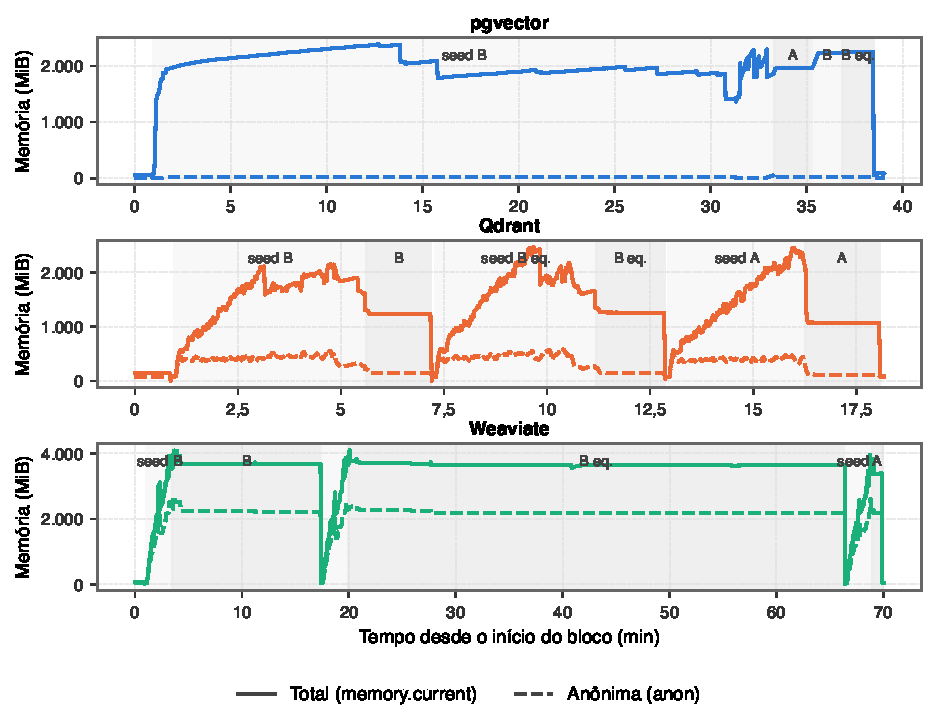
\includegraphics[width=\textwidth]{fig_memoria_500000}
\caption{Memória dos contêineres ao longo de cada bloco em 500k vetores. Mesmas convenções da Figura~\ref{fig:memoria_1m}.}
\label{fig:memoria_500k}
\end{figure}

\section{Repositório e reprodução}
\label{ap:repositorio}

O código do experimento, os arquivos de resultado e o texto deste relatório estão em um repositório público:

\begin{center}
\url{https://github.com/RNobre1/IC-Vetoriais}
\end{center}

A versão que corresponde a este relatório está marcada com a \textit{tag} \code{relatorio-final}, e a do relatório parcial, com \code{relatorio-parcial}. As tabelas, as figuras e os Códigos~\ref{cod:indice} e~\ref{cod:filtro} são gerados a partir do repositório pelo comando \code{make tabelas}; nenhum deles foi copiado à mão. A Tabela~\ref{tab:repositorio} indica onde está cada parte.

\begin{table}[H]
\centering
\caption{Organização do repositório.}
\label{tab:repositorio}
\renewcommand{\arraystretch}{1.15}
\small
\begin{tabularx}{\textwidth}{|l|X|}
\hline
\textbf{Caminho} & \textbf{Conteúdo} \\
\hline
\code{code/benchmarks/} & Cenários A, B e C, consultas de cada sistema (Código~\ref{cod:filtro}) e o executor da sessão de medição \\
\code{code/seeders/} & Carga dos vetores e criação do índice em cada sistema (Código~\ref{cod:indice}) \\
\code{code/ground\_truth/} & Busca exata usada como referência do \textit{recall} \\
\code{code/lib/} & Métricas, amostrador de recursos e gravação dos resultados \\
\code{code/analise/} & Geração das tabelas, das figuras e das listagens deste relatório \\
\code{code/results/} & Arquivos de resultado; \code{sessoes/2026-11-16-cpu-fixa/} guarda o ambiente, os marcos de fase e o registro do amostrador da sessão deste relatório \\
\code{code/tests/} & Testes unitários, executados pela integração contínua, e de integração \\
\code{docx/relatorio\_parcial/} & Fonte LaTeX deste relatório \\
\code{vault/decisões/} & Decisões de protocolo, registradas antes das medições \\
\hline
\end{tabularx}
\end{table}

A reprodução exige Docker com Compose, Python 3.11 e cerca de 16 GiB de memória para a escala de 1 milhão de vetores. A partir do diretório \code{code/}, \code{make deps} cria o ambiente Python com as dependências fixadas, \code{make up} sobe os três sistemas e \code{make sessao SESSAO\_ID=<nome>} executa a sessão completa descrita na Seção~\ref{sec:protocolo}, que recria os volumes antes de cada bloco. O MS MARCO é baixado no primeiro uso. Ao fim, \code{make tabelas} regenera o material do relatório a partir dos resultados. A fixação da frequência da CPU usa um comando com privilégio de administrador, descrito no roteiro de medição do repositório (\code{docs/runbook-medicao-dell.md}).

O código está sob a licença MIT. Os dados de medição, o texto e as figuras estão sob a licença Creative Commons Atribuição 4.0 Internacional (CC BY 4.0).
